\begin{figure}[H]
	\centering
	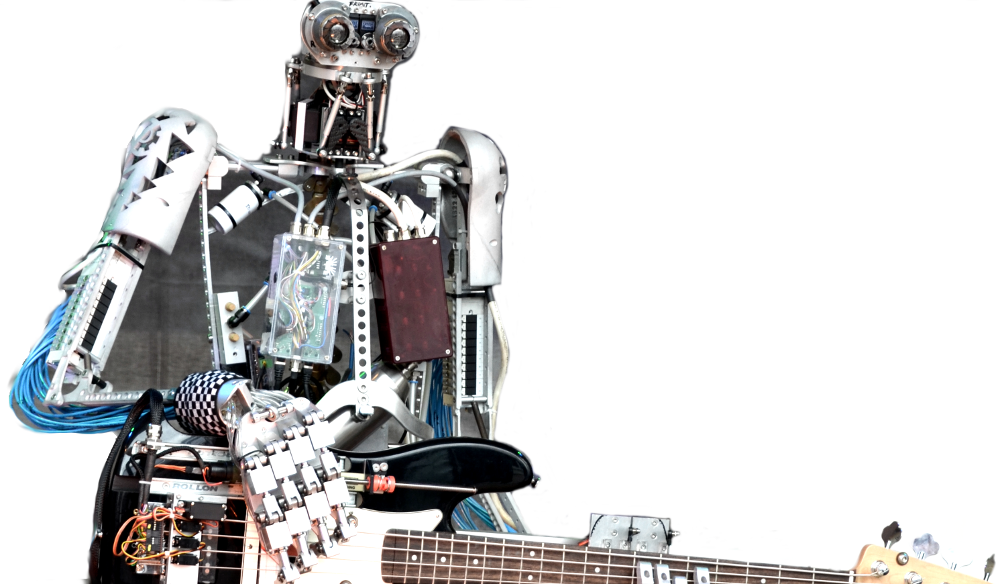
\includegraphics[scale=0.4]{img/chead.png}
\end{figure}
\begin{abstract}
Il progetto IMprovEEsation nasce dall'interesse degli autori, tutti musicisti, per la machine improvisation, un settore dell'intelligenza artificiale che mira a delineare le difficili sfumature dell'improvvisazione musicale da parte della macchina.
Questo progetto in realtà si discosta da tutte le attuali tematiche della machine improvisation, tentando di ricreare un ambiente nel quale i musicisti danno sfogo ai propri stili personali sotto sporadiche direttive: la Jam Session.
Più in particolare, il progetto mira a simulare, attraverso più agenti comunicanti, i diversi musicisti che prendono parte alla jam session e contribuiscono nel creare un brano che deve la sua origine soltanto alla definizione di relativamente pochi parametri.

Il report spiega dettagliatamente le tecniche, soprattutto di Intelligenza Artificiale, utilizzate per portare a un punto stabile (il proof of concept) tale progetto.
In particolare vi è un confronto fra due approcci utilizzati per definire il comportamento di un generico musicista: l'approccio stocastico, che segue pattern dati dalla conoscenza a priori dello stesso, e l'approccio evoluzionistico, che intende portare nuova conoscenza nelle azioni del musicista attraverso un algoritmo genetico e un ideale da seguire.

Logicamente, questo è un progetto in divenire, soprattutto perché non vi è una perfezione, né un modo procedurale per stabilire se un brano è corretto, ma è dettato dal gusto, come la stessa improvvisazione.
Nonostante ciò, la consideriamo un ottima prova del fatto che un tale traguardo è effettivamente possibile.
\end{abstract}
